\documentclass[intro-breve-latex.tex]{subfiles}
\begin{document}

\chapter{Escribir matemáticas}
\label{sec:maths}
\section{Básico}
\LaTeX{} admite dos formas de denotar matemáticas, en modo \textit{entre líneas} y modo \textit{display}. El primero se
escribe así \lstinline|$1+1=2$| $1+1=2$, mientras que el segundo se escribe así:
\begin{lstlisting}
$$ 1 + 1 = 2 $$
\end{lstlisting}
o también así \lstinline|\[ 1+1=2 \]|.
$$1+1=2$$
Esta distinción es importante, pues \LaTeX{} tomará ciertas decisiones para no interferir con el resto del texto, lo que
hará que el modo entre líneas tenga ciertas peculiaridades. Notemos que por defecto \LaTeX{} entiende que ha de añadir
espacios entre las operaciones, además los números no se inclinan mientras que las letras sí, e.g.\ 
\lstinline|$a\cdot a=a^2$| $a\cdot a=a^2$.

\LaTeX{} también admite subíndeces con \texttt{\_}, e.g., \lstinline|$x_1 \leq x_2$| $x_1 \leq x_2$, pero hemos de tener cuidado con los índices y las potencias pues \lstinline|$a^-1$| da $a^-1$, esto se debe a que \LaTeX{} sólo interpreta el primer símbolo arriba, algo similar ocurre con los índices; para usar más de uno juntos se pueden agrupar con \texttt{\{\}}, e.g. \lstinline|$\pi^{-1}$| $\pi^{-1}$.

Igual que con $\pi$, \LaTeX{} incluye comandos para varios otros símbolos usuales:
\begin{ltabular}{ll|ll}
	Griego \\
	\hline
	\lstinline|$\alpha A$|                & $\alpha A$                & \lstinline|$\nu N$|                & $\nu N$ \\
	\lstinline|$\beta B$|                 & $\beta B$                 & \lstinline|$\xi\Xi$|               & $\xi\Xi$ \\
	\lstinline|$\gamma \digamma \Gamma$|  & $\gamma \digamma \Gamma$  & \lstinline|$o O$|                  & $o O$ \\
	\lstinline|$\delta \Delta$|           & $\delta \Delta$           & \lstinline|$\pi\varpi\Pi$|         & $\pi\varpi\Pi$ \\
	\lstinline|$\epsilon \varepsilon E$|  & $\epsilon \varepsilon E$  & \lstinline|$\rho\varrho P$|        & $\rho\varrho P$ \\
	\lstinline|$\zeta Z$|                 & $\zeta Z$                 & \lstinline|$\sigma \Sigma$|        & $\sigma \Sigma$ \\
	\lstinline|$\eta H$|                  & $\eta H$                  & \lstinline|$\tau T$|               & $\tau T$ \\
	\lstinline|$\theta \vartheta \Theta$| & $\theta \vartheta \Theta$ & \lstinline|$\upsilon \Upsilon$|    & $\upsilon \Upsilon$ \\
	\lstinline|$\iota I$|                 & $\iota I$                 & \lstinline|$\phi \varphi \Phi$|    & $\phi \varphi \Phi$ \\
	\lstinline|$\kappa \varkappa K$|      & $\kappa \varkappa K$      & \lstinline|$\chi X$|               & $\chi X$ \\
	\lstinline|$\lambda \Lambda$|         & $\lambda \Lambda$         & \lstinline|$\psi \Psi$|            & $\psi \Psi$ \\
	\lstinline|$\mu M$|                   & $\mu M$                   & \lstinline|$\omega \Omega$|        & $\omega \Omega$ \\
	\hline
	Hebreo \\
	\hline
	\lstinline|$\aleph$| & $\aleph$ & \lstinline|$\beth$|   & $\beth$ \\
	\lstinline|$\gimel$| & $\gimel$ & \lstinline|$\daleth$| & $\daleth$ \\
	\hline
	Operaciones \\
	\hline
	\lstinline|$\cdot$|     & $\cdot$     & \lstinline|$\times$|    & $\times$ \\
	\lstinline|$\pm$|       & $\pm$       & \lstinline|$\mp$|       & $\mp$ \\
	\lstinline|$\div$|      & $\div$      & \lstinline|$\star$|     & $\star$ \\
	\lstinline|$\cap$|      & $\cap$      & \lstinline|$\cup$|      & $\cup$ \\
	\lstinline|$\sqcap$|    & $\sqcap$    & \lstinline|$\sqcup$|    & $\sqcup$ \\
	\lstinline|$\neq$|      & $\neq$      & \lstinline|$\setminus$| & $\setminus$ \\
	\lstinline|$\leq$|      & $\leq$      & \lstinline|$\geq$|      & $\geq$ \\
	\lstinline|$\ll$|       & $\ll$       & \lstinline|$\gg$|       & $\gg$ \\
	\lstinline|$\lhd$|      & $\lhd$      & \lstinline|$\rhd$|      & $\rhd$ \\
	\lstinline|$\unlhd$|    & $\unlhd$    & \lstinline|$\unrhd$|    & $\unrhd$ \\
	\lstinline|$\in$|       & $\in$       & \lstinline|$\perp$|     & $\perp$ \\
	\lstinline|$\mid$|      & $\mid$      & \lstinline|$\parallel$| & $\parallel$ \\
	\lstinline|$\notin$|    & $\notin$    & \lstinline|$\subset$|   & $\subset$ \\
	\lstinline|$\subseteq$| & $\subseteq$ & \lstinline|$\supseteq$| & $\supseteq$ \\
	\lstinline|$\prec$|     & $\prec$     & \lstinline|$\succ$|     & $\succ$ \\
	\lstinline|$\preceq$|   & $\preceq$   & \lstinline|$\succeq$|   & $\succeq$ \\
	\lstinline|$\simeq$|    & $\simeq$    & \lstinline|$\approx$|   & $\approx$ \\
	\lstinline|$\asymp$|    & $\asymp$    & \lstinline|$\propto$|   & $\propto$ \\
	\lstinline|$\wedge$|    & $\wedge$    & \lstinline|$\vee$|      & $\vee$ \\
	\lstinline|$\oplus$|    & $\oplus$    & \lstinline|$\otimes$|   & $\otimes$ \\
	\lstinline|$\odot$|     & $\odot$     & \lstinline|$\ominus$|   & $\ominus$ \\
	\lstinline|$\circ$|     & $\circ$     & \lstinline|$\sim$|      & $\sim$ \\
	\lstinline|$\equiv$|    & $\equiv$    & \lstinline|$\cong$|     & $\cong$ \\
	\lstinline|$\smile$|    & $\smile$    & \lstinline|$\frown$|    & $\frown$ \\
	\lstinline|$\to$|       & $\to$       & \lstinline|$\implies$|  & $\implies$ \\
	\hline
	Delimitadores \\
	\hline
	\lstinline!$|$!                   & $|$                   & \lstinline!$\|$!                  & $\|$ \\
	\lstinline!$\lvert a\rvert$!      & $\lvert a\rvert$      & \lstinline!$\lVert a\rVert$!      & $\lVert a\rVert$ \\
	\lstinline|$\{\}$|                & $\{\}$                & \lstinline|$\lfloor \rfloor$|     & $\lfloor \rfloor$ \\
	\lstinline|$\lceil \rceil$|       & $\lceil \rceil$       & \lstinline|$\langle \rangle$|     & $\langle \rangle$ \\
	\lstinline|$\ulcorner \urcorner$| & $\ulcorner \urcorner$ & \lstinline|$\llcorner \lrcorner$| & $\llcorner \lrcorner$ \\
	\hline
	Acentos \\
	\hline
	\lstinline|$\vec{a}$|    & $\vec{a}$    & \lstinline|$\overrightarrow{ab}$|  & $\overrightarrow{ab}$ \\
	\lstinline|$\dot{a}$|    & $\dot{a}$    & \lstinline|$\ddot{a}$|             & $\ddot{a}$ \\
	\lstinline|$\hat{a}$|    & $\hat{a}$    & \lstinline|$\widehat{ab}$|         & $\widehat{ab}$ \\
	\lstinline|$\bar{a}$|    & $\bar{a}$    & \lstinline|$\overline{ab}$|        & $\overline{ab}$ \\
	\lstinline|$\acute{a}$|  & $\acute{a}$  & \lstinline|$\grave{a}$|            & $\grave{a}$ \\
	\lstinline|$\check{a}$|  & $\check{a}$  & \lstinline|$\breve{a}$|            & $\breve{a}$ \\
	\hline
	Otros \\
	\hline
	\lstinline|$\infty$|       & $\infty$       & \lstinline|$\forall$|     & $\forall$ \\
	\lstinline|$\Re$|          & $\Re$          & \lstinline|$\Im$|         & $\Im$ \\
	\lstinline|$\nabla$|       & $\nabla$       & \lstinline|$\exists$|     & $\exists$ \\
	\lstinline|$\partial$|     & $\partial$     & \lstinline|$\nexists$|    & $\nexists$ \\
	\lstinline|$\emptyset$|    & $\emptyset$    & \lstinline|$\varnothing$| & $\varnothing$ \\
	\lstinline|$\wp$|          & $\wp$          & \lstinline|$\complement$| & $\complement$ \\
	\lstinline|$\neg$|         & $\neg$         & \lstinline|$\aleph$|      & $\aleph$ \\
	\lstinline|$\square$|      & $\square$      & \lstinline|$\surd$|       & $\surd$ \\
	\lstinline|$\blacksquare$| & $\blacksquare$ & \lstinline|$\triangle$|   & $\triangle$ \\
	\lstinline|$\diamond$|     & $\diamond$     & \lstinline|$\bullet$|     & $\bullet$ \\
\end{ltabular}

Para los marcados con violeta, se requieren dos nuevos paquetes:
\begin{lstlisting}
\usepackage{amsmath, amssymb}
\end{lstlisting}
Nótese que al estar separados por coma, \LaTeX{} entiende que son dos paquetes independientes. Si no le interesan dichos símbolos aun se recomienda importar el primero.

\textbf{Encontrar símbolos.}
En general es una tarea practicamente imposible la de aprenderse de memoria todos los símbolos en \LaTeX{}, sin
considerar el hecho de que ciertos paquetes importan cada vez más de ellos, por lo que se recomienda con creces usar
este sitio web \url{http://detexify.kirelabs.org/classify.html} donde puedes encontrar símbolos mediante dibujos. Bajo
el comando donde aparecen se especifica si el comando funciona en modo texto o modo matemático (o ambos), y arriba
especificará si requiere algún paquete.

Otra observación es que si bien \lstinline!|! sirve y genera el mismo efecto en modo matemático que \lstinline|\mid|, el
primero se recomienda como \textit{envoltura} (similar a los paréntesis), mientras que el segundo genera espacios como
para el <<divide a>>, e.g., \lstinline!$|x|; 2\mid 4$! $|x|; 2\mid 4$.
Esta distinción aplica para el resto de delimitadores.

\textbf{Puntos.}
En \LaTeX{} hay distintos tipos de puntos: centrados, bajos, verticales y diagonales (del tipo \smash{$\ddots$}).
Para ello se escribe el punto centrado solo como \lstinline|$\cdot$| como hemos visto, pero los tres juntos se escriben
\lstinline|$\cdots, \dots, \vdots, \ddots$| \smash{$\cdots, \dots, \vdots, \ddots$} respectivamente.

Como recomendación se usa los puntos centrados para operaciones, e.g., \lstinline|$1+2+\cdots+99+100$|
$1+2+\cdots+99+100$, y los bajos para listas \lstinline|$\{ 1, 2, \dots, 100 \}$| $\{1,2,\dots,100\}$.

También están incorporados los lógicos \lstinline|$\because$| $\because$ y \lstinline|$\therefore$| $\therefore$ (con
\AmS{}). Y el comando \lstinline|$\colon$| especialmente hecho para funciones\break \lstinline|$f\colon A \to B$| $f\colon A \to B$.

\textbf{Fracciones.}
Para hacer fracciones existe el comando \lstinline|\frac| que funciona como:
\begin{lstlisting}
$$ \frac{1}{2} + \frac{1}{3} = \frac{5}{6}. $$
\end{lstlisting}
$$ \frac{1}{2} + \frac{1}{3} = \frac{5}{6}. $$
No obstante, el comando cambia si estamos en modo texto: \lstinline|$\frac{22}{7}$| $\frac{22}{7}$ y también lo hace si ponemos varias fracciones juntas:
\begin{lstlisting}[basicstyle=\scriptsize\ttfamily]
$$ \frac{1}{1 + \frac{1}{1 + \frac{1}{1 + \frac{1}{\ddots}}}} $$
\end{lstlisting}
$$ \frac{1}{1 + \frac{1}{1 + \frac{1}{1 + \frac{1}{\ddots}}}} $$
Esto se debe a que en el numerador y denominador se pasa a modo entre líneas para no ocupar demasiado espacio, en el modo entre líneas se utiliza para que las líneas se mantengan constantes en altura, no obstante, de ser necesario puede usar \lstinline|\dfrac| para forzar una fracción en modo \textit{display} y \lstinline|\tfrac| para forzar modo entre líneas.
\begin{lstlisting}[basicstyle=\scriptsize\ttfamily]
$$ \dfrac{1}{1 + \dfrac{1}{1 + \dfrac{1}{1 + \dfrac{1}{\ddots}}}} $$
\end{lstlisting}
$$ \dfrac{1}{1 + \dfrac{1}{1 + \dfrac{1}{1 + \dfrac{1}{\ddots}}}} $$
\begin{lstlisting}[basicstyle=\scriptsize\ttfamily]
$$ \frac{2}{5} + \frac{39}{45} = \frac{57}{45} = 1\tfrac{12}{45} $$
\end{lstlisting}
$$ \frac{2}{5} + \frac{39}{45} = \frac{57}{45} = 1\tfrac{12}{45} $$
Un comando similar es \lstinline|\binom| que genera coeficientes binomiales, e.g.,\break
\lstinline|$\binom{3}{2}$| $\binom{3}{2}$.
Al igual que \lstinline|\frac| admite las variaciones \lstinline|\dbinom| y \lstinline|\tbinom|.

% \textbf{Congruencias modulares.}
% Para módulos hay una serie de comandos distintos:
% \begin{lstlisting}
% $$ (-1)^{ 5\bmod 2 }, \quad 5\equiv 2 \pmod 3,
% \quad 7\equiv 3 \mod 4, \quad 5\equiv 1 \pod 4. $$
% \end{lstlisting}
% $$ (-1)^{ 5\bmod 2 }, \quad 5\equiv 2 \pmod 3,
% \quad 7\equiv 3 \mod 4, \quad 5\equiv 1 \pod 4. $$
% Nótese que \lstinline|\bmod| no genera espacios anteriores, en cambio \lstinline|\mod| sí.

\textbf{Raíces.}
Este es muy sencillo, así se describe una raíz cuadrada \lstinline|$\sqrt{17}$| $\sqrt{17}$, y así una raíz $n$-ésima
\lstinline|$\sqrt[3]{8} = 2$| $\sqrt[3]{8} = 2$.

\textbf{Operadores.}
En general a los símbolos destinados a ir entre dos caracteres como + se les dice <<operación binaria>>, por separado,
un operador es una palabra o frase que se utiliza expicitamente y, por lo general, en letras romanas derechas; e.g.,
\lstinline|$\sin x$| $\sin x$.

Los operadores se clasifican en dos: grandes o pequeños, donde ambos ocupan el mismo tamaño para su nombre, pero los
grandes tienen la gracia de que sus subíndices y superíndices van directamente abajo y arriba respectivamente del
nombre, por ejemplo:
\begin{lstlisting}
$$ \lim_{x \to \infty} \sin^2 x + \cos^2 x = 1. $$
\end{lstlisting}
$$ \lim_{x \to \infty} \sin^2 x + \cos^2 x = 1. $$
Aquí \lstinline|\sin,\cos| son pequeños mientras que \lstinline|\lim| es grande.

Los operadores no siempre tienen que tener texto, pueden poseer otros símbolos como:
\begin{lstlisting}[basicstyle=\footnotesize\ttfamily]
$$ \sum_{i=0}^n i = \frac{n(n+1)}{2}, \int_a^b f(x) dx. $$
\end{lstlisting}
$$ \sum_{i=0}^n i = \frac{n(n+1)}{2}, \int_a^b f(x) dx. $$
Cabe notar que dicha característica de los operadores grande se pierde en el modo entre líneas, e.g.,
\lstinline|$\prod_{k=1}^n i = n!$| $\prod_{k=1}^n i = n!$
\begin{longtable}{llll}
	\hline \hline
	\endhead
	\hline \hline
	\endfoot

	\lstinline|$\sin$|    & $\sin$    & \lstinline|$\sinh$|   & $\sinh$ \\
	\lstinline|$\cos$|    & $\cos$    & \lstinline|$\cosh$|   & $\cosh$ \\
	\lstinline|$\tan$|    & $\tan$    & \lstinline|$\tanh$|   & $\tanh$ \\
	\lstinline|$\arcsin$| & $\arcsin$ & \lstinline|$\csc$|    & $\csc$  \\
	\lstinline|$\arccos$| & $\arccos$ & \lstinline|$\sec$|    & $\sec$  \\
	\lstinline|$\arctan$| & $\arctan$ & \lstinline|$\cot$|    & $\cot$  \\

	\lstinline|$\deg$|    & $\deg$    & \lstinline|$\dim$|    & $\dim$ \\
	\lstinline|$\arg$|    & $\arg$    & \lstinline|$\exp$|    & $\exp$ \\
	\lstinline|$\hom$|    & $\hom$    & \lstinline|$\ker$|    & $\ker$ \\
	\lstinline|$\lg$|     & $\lg$     & \lstinline|$\ln$|     & $\ln$ \\
	\lstinline|$\log$|    & $\log$    &  \\
	\hline
	\lstinline|$\liminf$|    & $\liminf$    & \lstinline|$\limsup$|     & $\limsup$ \\
	\lstinline|$\varliminf$| & $\varliminf$ & \lstinline|$\varlimsup$|  & $\varlimsup$ \\
	\lstinline|$\injlim$|    & $\injlim$    & \lstinline|$\projlim$|    & $\projlim$ \\
	\lstinline|$\varinjlim$| & $\varinjlim$ & \lstinline|$\varprojlim$| & $\varprojlim$ \\

	\lstinline|$\inf$|      & $\inf$      & \lstinline|$\sup$|       & $\sup$ \\
	\lstinline|$\min$|      & $\min$      & \lstinline|$\max$|       & $\max$ \\
	\lstinline|$\lim$|      & $\lim$      & \lstinline|$\gcd$|       & $\gcd$ \\
	\lstinline|$\Pr$|       & $\Pr$       & \lstinline|$\det$|       & $\det$ \\
	\lstinline|$\int$|      & $\int$      & \lstinline|$\iint$|      & $\iint$ \\
	\lstinline|$\iiint$|    & $\iiint$    & \lstinline|$\idotsint$|  & $\idotsint$ \\
	\lstinline|$\oint$|     & $\oint$     & \lstinline|$\coprod$|    & $\coprod$ \\
	\lstinline|$\sum$|      & $\sum$      & \lstinline|$\prod$|      & $\prod$ \\
	\lstinline|$\bigcup$|   & $\bigcup$   & \lstinline|$\bigcap$|    & $\bigcap$ \\
	\lstinline|$\bigsqcup$| & $\bigsqcup$ & \lstinline|$\biguplus$|  & $\biguplus$ \\
	\lstinline|$\bigvee$|   & $\bigvee$   & \lstinline|$\bigwedge$|  & $\bigwedge$ \\
	\lstinline|$\bigoplus$| & $\bigoplus$ & \lstinline|$\bigotimes$| & $\bigotimes$ \\
	\lstinline|$\bigodot$|  & $\bigodot$  \\
\end{longtable}

En la lista los primeros son los pequeños y los segundos los grandes.
Los violetas requieren de paquetes tipo \AmS{}.

\textbf{Operadores modulares.} Para \LaTeX{} existen cuatro tipos de operadores modulares:
\begin{lstlisting}
\begin{align*}
	3 &\equiv 1 \pmod 2, & 3 &\equiv 1 \pod 2, \\
	3 &\equiv 1  \mod 2, & \bmod(3, 2) &= 1.
\end{align*}
\end{lstlisting}
\begin{align*}
	3 &\equiv 1 \pmod 2, & 3 &\equiv 1 \pod 2, \\
	3 &\equiv 1  \mod 2, & \bmod(3, 2) &= 1.
\end{align*}

\textbf{Definir operadores.} Para definir operaciones se debe utilizar el comando \lstinline|\DeclareMathOperator{¬com¬}{¬tag¬}| en la cabecera. Si se declara con un \texttt{*} antes de las llaves, entonces se definirá un operador grande, e.g:
\begin{lstlisting}
\DeclareMathOperator{\mcd}{mcd}
\DeclareMathOperator*{\dom}{dom}
------------------------------------------------
$$ \mcd(21, 70) = 7,\quad \dom_V(f) = A. $$
\end{lstlisting}
$$ \mcd(21, 70) = 7,\quad \dom_V(f) = A. $$
Pero esto es una definición general, aquí defines un comando para todo el documento lo que puede o no ser de su agrado, si tiene un operador que desea ocupar una única vez entonces es más recomendable usar \lstinline|\operatorname|; sus efectos son los mismos:
\begin{lstlisting}
$$ \operatorname{mcm}(3, 16) = 48,\quad \operatorname*{cod}_V(f) = B. $$
\end{lstlisting}
$$ \operatorname{mcm}(3, 16) = 48,\quad \operatorname*{cod}_V(f) = B. $$
También podemos utilizar el anterior para redefinir comandos, por ejemplo si no nos gusta que \lstinline|$\Re, \Im$| se vean así $\Re, \Im$, podemos poner esto en la cabecera:
\begin{lstlisting}
\renewcommand{\Re}{\operatorname{Re}}
\renewcommand{\Im}{\operatorname{Im}}
\end{lstlisting}
Para que se vean así $\operatorname{Re}, \operatorname{Im}$.

\textbf{Espacios.}
El ejemplo anterior también sirve para ilustrar una característica del modo matemático, la cual es que no lee los
espacios singulares del código, e.g., \lstinline|$a     b$| genera $a     b$. Para añadir espacios también hay comandos
singulares:
\begin{figure}[!h]
	\centering
	\begin{longtable}{ll}
		\hline \hline
		\endhead
		\hline \hline
		\endfoot

		\lstinline|$a\!b$|      & $a\!b$ \\
		\lstinline|$ab$|        & $ab$ \\
		\lstinline|$a\,b$|      & $a\,b$ \\
		\lstinline|$a\;b$|      & $a\;b$ \\
		\lstinline|$a\ b$|      & $a\ b$ \\
		\lstinline|$a\quad b$|  & $a\quad b$ \\
		\lstinline|$a\qquad b$| & $a\qquad b$ \\
	\end{longtable}
\end{figure}

\textbf{Fuentes de letras.} Para el modo matemático también hay fuentes de letras:
\begin{center}
	\begin{longtable}{lp{8cm}}
		\hline \hline
		\endhead
		\hline \hline
		\endfoot

		\lstinline|\mathrm|   & $\mathrm{ABCDEFGHIJKLMNOPQRSTUVWXYZ}$ $\mathrm{abcdefghijklmnopqrstuvwxyz}$ $\mathrm{1234567890}$ \\
		\lstinline|\mathbf|   & $\mathbf{ABCDEFGHIJKLMNOPQRSTUVWXYZ}$ $\mathbf{abcdefghijklmnopqrstuvwxyz}$ $\mathbf{1234567890}$ \\
		\lstinline|\mathsf|   & $\mathsf{ABCDEFGHIJKLMNOPQRSTUVWXYZ}$ $\mathsf{abcdefghijklmnopqrstuvwxyz}$ $\mathsf{1234567890}$ \\
		\lstinline|\mathcal|  & $\mathcal{ABCDEFGHIJKLMNOPQRSTUVWXYZ}$ \\
		\lstinline|\mathbb|   & $\mathbb{ABCDEFGHIJKLMNOPQRSTUVWXYZ}$ \\
		\lstinline|\mathfrak| & $\mathfrak{ABCDEFGHIJKLMNOPQRSTUVWXYZ}$ $\mathfrak{abcdefghijklmnopqrstuvwxyz}$ $\mathfrak{1234567890}$ \\
		\lstinline|\mathscr|  & $\mathscr{ABCDEFGHIJKLM}$ $\mathscr{NOPQRSTUVWXYZ}$ \\
	\end{longtable}
\end{center}
La fuente \lstinline|\mathbb| viene con \AmS{}, \lstinline|\mathfrak| con el paquete \texttt{eufrak} y\break
\lstinline|\mathscr| con \texttt{mathrsfs}.

Es común usar la tipografía \lstinline|\mathbb| para conjuntos numéricos famosos como \lstinline|$\mathbb{N}$| $\mathbb{N}$. A veces,
éstos suelen ser tan comúnes y conocidos, que suele ser útil definir un comando para ellos:
\begin{lstlisting}
\newcommand{\N}{\mathbb{N}}
\newcommand{\Z}{\mathbb{Z}}
\newcommand{\Q}{\mathbb{Q}}
\newcommand{\R}{\mathbb{R}}
\newcommand{\C}{\mathbb{C}}
\end{lstlisting}
\textbf{Texto en ecuaciones.}
Si bien la fuente \lstinline|\mathrm| es la misma del texto del documento, todavía tendríamos que lidiar con los
espacios del modo matemático sin hablar de que no admiten caracteres \texttt{utf-8} (i.e., cosas como \lstinline|$á$|
generan errores), pero \LaTeX{} admite texto en ecuaciones, sólo basa usar \lstinline|\text|, e.g.
\lstinline|$x=2,\text{ mientras que }y=3$| $x=2,\text{ mientras que }y=3$. Esto es más útil en ecuaciones en modo
\textit{display}.

\section{Ecuaciones numeradas, alineadas, matrices y más}
\textbf{Ecuaciones numeradas.} Hasta ahora nuestras ecuaciones no están numeradas, ni poseen un número para añadirlas, para hacerlo debes usar el entorno \texttt{equation}. Dentro de él se permiten el uso de referencias cruzadas, respecto a esto se recomienda usar \lstinline|\eqref| en lugar de \lstinline|\ref| por estética, aunque sus usos son iguales, e.g:
\begin{lstlisting}
...y así se deduce el llamado \textit{teorema de Pitágoras} \eqref{eq:pitagoras}:
\begin{equation} \label{eq:pitagoras}
	a^2 + b^2 = c^2
\end{equation}
\end{lstlisting}
...y así se deduce el llamado \textit{teorema de Pitágoras} \eqref{eq:pitagoras}:
\begin{equation} \label{eq:pitagoras}
	a^2 + b^2 = c^2
\end{equation}

Como se ve, \LaTeX{} automáticamente enumera la ecuación como \ref{eq:pitagoras}, si se quiere cambiar dicho tag se puede mediante el comando \lstinline|\tag|, e.g:
\begin{lstlisting}
\begin{equation}\label{eq:einstein}
	E = mc^2 \tag{Ein}
\end{equation}
Y \eqref{eq:einstein} es la famosa fórmula de Einstein...
\end{lstlisting}

\begin{equation}\label{eq:einstein}
	E = mc^2 \tag{Ein}
\end{equation}
Y \eqref{eq:einstein} es la famosa fórmula de Einstein...

Además se puede quitar los tags con \lstinline|\notag|, que tal vez no es útil aún, pero lo será pronto.

\textbf{Ecuaciones alineadas.}
Es común ver documentos donde una ecuación está alineada por signos ``$=$'' y no saber como, además notará que entre
\lstinline|$$ ... $$| no funcionan los cortes de línea. Para ello existe el entorno \texttt{align} y \texttt{align*}.
Donde las partes son como celdas de una tabla y se separan por \texttt{\&}. El primero enumera cada línea, mientras que
el segundo no enumera ninguna, e.g:
\begin{lstlisting}[basicstyle=\footnotesize\ttfamily, tabsize=4]
\begin{align}
	\sum_{i=1}^n i &= 1 + 2 + 3 + \cdots + (n-1) + n \notag \\
	&= (1 + n) + (2 + (n-1)) + (3 + (n-2)) + \cdots \notag \\
	&= (n+1) + (n+1) + (n+1) + \cdots \notag \\
	&= (n+1)\cdot\frac{n}{2} = \frac{n(n+1)}{2}.
\end{align}
\end{lstlisting}
\begin{align}
	\sum_{i=1}^n i &= 1 + 2 + 3 + \cdots + (n-1) + n \notag \\
	&= (1 + n) + (2 + (n-1)) + (3 + (n-2)) + \cdots \notag \\
	&= (n+1) + (n+1) + (n+1) + \cdots \notag \\
	&= (n+1)\cdot\frac{n}{2} = \frac{n(n+1)}{2}.
\end{align}
Un detalle importante es que por defecto \LaTeX{} no rompe una ecuación alineada entre páginas, sin importar cuan larga
sea, si usted quiere permitir esto debe agregar este comando a la cabecera:
\begin{lstlisting}
\allowdisplaybreaks
\end{lstlisting}
Otra necesidad puede ser la de poner texto entre igualdades, para lo cual se emplea \lstinline|\intertext{}|:
% \begin{lstlisting}
% \allowdisplaybreaks
% \end{lstlisting}
% \begin{align*}
% 	\intertext{empleando que la serie converge absolutamente, podemos intercambiar sumatorias}
% 	&= 
% \end{align*}

\textbf{Ecuaciones multilíneas.}
Ésta es diferente de la anterior, en esta se usan varias líneas, pero todos bajo un mismo número, o varias ecuaciones,
pero sin alinear. Para una ecuación muy larga se puede usar el entorno \texttt{multline} y para varias ecuaciones
no-alineadas el entorno \texttt{gather}. El asterisco indica si van enumeradas o no:
\begin{lstlisting}
\begin{multline*}
	f(x) = 59x^{11} + 86x^{10} + 22x^9 + 83x^8 + 74x^7 + 49x^6 + 12x^5 + 83x^4\\
	+ 42x^3 + 69x^2 + 47x + 93.
\end{multline*}
y
\begin{gather*}
	g(x) = 47x^2 + 62x + 45\\
	h(x) = 18x^5 + 21x^3 + 61x - 9
\end{gather*}
\end{lstlisting}
\begin{multline*}
	f(x) = 59x^{11} + 86x^{10} + 22x^9 + 83x^8 + 74x^7 + 49x^6 + 12x^5 + 83x^4\\
	+ 42x^3 + 69x^2 + 47x + 93.
\end{multline*}
y
\begin{gather*}
	g(x) = 47x^2 + 62x + 45\\
	h(x) = 18x^5 + 21x^3 + 61x - 9
\end{gather*}

\textbf{Modo entre-línea, display y \textit{smash}.} A mucha gente le molesta el hecho de que \LaTeX{} achica ciertos símbolos para mantener constancia en sus líneas, en cosas como $\sum_{k=1}^n k$ y otros operadores grandes. Ya vimos el problema con \lstinline|\dfrac|, pero no vimos el caso general para \lstinline|\lim| y el resto de operadores grandes. Para esto \LaTeX{} posee los \underline{modificadores} \lstinline|\displaystyle| y \lstinline|\textstyle| que fuerzan el modo display y entre-líneas respectivamente en cualquier entorno. Personalmente no recomiendo esto por mal uso de líneas, e.g. \lstinline|$\displaystyle \sum_{k=1}^n k$| $\displaystyle \sum_{k=1}^n k$ provoca malos espacios; no obstante hay casos donde se podría hacer sin afectar el espacio, para ello está el comando \lstinline|\smash|:
\begin{lstlisting}[basicstyle=\footnotesize\ttfamily]
Línea corta. \\
Así que ahora podemos usar \smash{$\displaystyle\sum_{k=1}^n k$}. \\
Línea corta.
\end{lstlisting}
Línea corta. \\
Así que ahora podemos usar \smash{$\displaystyle\sum_{k=1}^n k$}. \\
Línea corta.

\textbf{Delimitadores grandes.} Otro problema de tamaño es que por defecto los delimitadores no se adaptan al tamaño de símbolos grandes en \LaTeX{}, e.g., $(\dfrac{1}{2})$ que se ve mal. Para ello se recomienda usar \lstinline|\left| y \lstinline|\right|, e.g. \lstinline|$\left(\dfrac{1}{2}\right)$| $\left(\dfrac{1}{2}\right)$. Estos se adaptan a cualquier símbolo, sin importar que tan grande, sólo se debe ser cuidadoso, \textbf{no se puede} usar \lstinline|\left| y luego no ocupar un \lstinline|\right| en la misma línea. En caso de que sólo se quiera usar un delimitador se debe poner un `\texttt{.}' en el otro, e.g:
\begin{lstlisting}
$$ \int_0^2 x^2\,dx = \left.\frac{x^3}{3}\right|_0^2 = \frac{8}{3}. $$
\end{lstlisting}
$$ \int_0^2 x^2\,dx = \left.\frac{x^3}{3}\right|_0^2 = \frac{8}{3}. $$
Para cambiar el tamaño de forma manual puede usar los siguientes:
\begin{center}
	\begin{tabular}{ll|ll}
		\hline \hline
		\lstinline|$\big($|  & $\big($  & \lstinline|$\Big($|  & $\Big($ \\
		\lstinline|$\bigg($| & $\bigg($ & \lstinline|$\Bigg($| & $\Bigg($ \\
		\hline \hline
	\end{tabular}
\end{center}

\textbf{Matrices.} Para escribir matrices, el paquete \texttt{amsmath} incluye el entorno \texttt{matrix} para el modo matemático que funciona como una tabla:
\begin{lstlisting}
$$ \mathbf{Id} :=
	\left[ \begin{matrix}
		1 & 0 \\
		0 & 1
	\end{matrix} \right] $$
\end{lstlisting}
$$ \mathbf{Id} :=
	\left[ \begin{matrix}
		1 & 0 \\
		0 & 1
	\end{matrix} \right] $$
Por defecto, el entorno no posee delimitadores, pero existen variaciones de él que sí:
\begin{center}
	\begin{tabular}{lc|lc}
		\hline \hline
		\texttt{matrix}  & {$\begin{matrix}  1 & 0 \\ 0 & 1 \end{matrix}$}  & \texttt{pmatrix} & {$\begin{pmatrix} 1 & 0 \\ 0 & 1 \end{pmatrix}$} \\[1.2em]
		\texttt{bmatrix} & {$\begin{bmatrix} 1 & 0 \\ 0 & 1 \end{bmatrix}$} & \texttt{Bmatrix} & {$\begin{Bmatrix} 1 & 0 \\ 0 & 1 \end{Bmatrix}$} \\[1.2em]
		\texttt{vmatrix} & {$\begin{vmatrix} 1 & 0 \\ 0 & 1 \end{vmatrix}$} & \texttt{Vmatrix} & {$\begin{Vmatrix} 1 & 0 \\ 0 & 1 \end{Vmatrix}$} \\
		\hline \hline
	\end{tabular}
\end{center}

\textbf{Teoremas.} Los teoremas en \LaTeX{} se importan con el paquete \texttt{amsthm}, funcionan como entornos que se numeran automáticamente y poseen otras cualidades, se definen en la cabecera así:
\begin{lstlisting}
\newtheorem{thm}{Teorema}
---------------------------------------------------
\begin{thm}
	La suma en $\mathbb{R}$ conmuta.
\end{thm}
\end{lstlisting}
\begin{thm}
	La suma en $\mathbb{R}$ conmuta.
\end{thm}
En este caso el teorema se enumeró sólo, podemos desactivar la numeración con \lstinline|\newtheorem*|. También el teorema partió desde el 1, pero podría haber iniciado ``\ref{sec:maths}.1'' donde el \ref{sec:maths} es el número de sección, o podría usar el número del capítulo en un libro, para ello le agregamos al final un campo opcional diciendo \texttt{section} o \texttt{chapter} lo que indica que la numeración se da en dicho formato. Algo interesante es que varios teoremas pueden compartir la misma numeración:
\begin{lstlisting}
\newtheorem{mydef}{Definición}[section]
\newtheorem{cor}[mydef]{Corolario}
\newtheorem*{note}{Observación}
---------------------------------------------------
\begin{mydef}[Hipotenusa y catetos]
	En un triángulo rectángulo, el lado opuesto al ángulo recto se dice \textit{hipotenusa} y el resto catetos.
\end{mydef}
\begin{note}
	Creo que recuerdo un teorema acerca de eso...
\end{note}
\begin{cor}
	La hipotenusa es mayor que los catetos.
\end{cor}
\end{lstlisting}
\begin{mydef}[Hipotenusa y catetos]
	En un triángulo rectángulo, el lado opuesto al ángulo recto se dice \textit{hipotenusa} y el resto catetos.
\end{mydef}
\begin{note}
	Creo que recuerdo un teorema acerca de eso...
\end{note}
\begin{cor}
	La hipotenusa es mayor que los catetos.
\end{cor}
\textbf{¡Precaución!} El paquete ya introduce un entorno para definiciones, así que no puede definir otro teorema también de tag \texttt{def}, por eso se usa \texttt{mydef}.

Por último cabe mencionar que los teoremas también permiten el uso de referencias cruzadas.

Y otros errores comúnes:
\begin{longtable}{|ll|ll|}
	\hline
	Código & Peor & Código & Mejor \\
	\hline
	\endhead

	\hline
	\endfoot

	\lstinline|$sin x$| & $sin x$ & \lstinline|$\sin x$| & $\sin x$ \\
	\lstinline?$||\vec v||$? & $||\vec v||$ & \lstinline?$\|\vec v\|$? & $\|\vec v\|$ \\
	\lstinline?$|-1|$? & $|-1|$ & \lstinline|$\lvert-1\rvert$| & $\lvert-1\rvert$ \\
	\lstinline?$<x, y>$? & $<x, y>$ & \lstinline?$\langle x, y\rangle$? & $\langle x, y\rangle$ \\
	\lstinline?$(\frac{1}{2})$? & $\displaystyle (\frac{1}{2}) $ & \lstinline|$\left(\frac{1}{2}\right)$| & $\displaystyle \left(\frac{1}{2}\right) $ \\
	\lstinline?$2 | 6$? & $2 | 6$ & \lstinline|$2 \mid 6$| & $2 \mid 6$ \\
	\lstinline?$r \| s$? & $r \| s$ & \lstinline|$r \parallel s$| & $r \parallel s$ \\
	\lstinline|$\int x dx$| & $\int x dx$ & \lstinline|$\int x\, dx$| & $\int x\, dx$ \\
	\lstinline|$f: A\to B$| & $f: A\to B$ & \lstinline|$f\colon A\to B$| & $f\colon A\to B$ \\
\end{longtable}

\section{Diagramas (básico)}
\textbf{¿Por qué?} Habiendo programas como GeoGebra, Photoshop y muchos más para hacer diagramas de forma fácil y gráfica, ¿por qué hacer diagramas en \LaTeX{} si es código? La razón es que \LaTeX{} fue hecho para la publicación de textos y para ello ocupa figuras vectoriales, esto genera el efecto de acercarse a los caracteres y no tener perdida de calidad.
Las imágenes en \LaTeX{} comparten esa misma cualidad y en ciertos casos, su facilidad de uso es comparable a la de un editor gráfico, y si no, hay editores que permiten exportar sus diagramas a \LaTeX{} (GeoGebra exporta a Ti$k$Z). Sin contar el que reduce el espacio utilizado en el archivo final y que puede resultar satisfactorio poder hacer figuras sin salir de \LaTeX{}.

Aquí, \texttt{width} determina el tamaño del gráfico (sin contar aquel espacio extra que ocupen los números, las etiquetas de los ejes y el título del gráfico). \texttt{samples} determina cuantos puntos de ejemplo tomar (más es mejor, pero puede retrasar la compilación, 100 es recomendable). El comando \lstinline|\addplot| añade un gráfico y en las opciones vimos que el dominio se determina por \lstinline|domain=¬i:f¬|. Además añadimos entradas por \lstinline|\addlegendentry|.

Para cambiar el grosor de cada gráfico se ocupan las siguientes opciones: \texttt{very thin}, \texttt{thin}, \texttt{thick} y \texttt{very thick}. Además se puede usar la opción \texttt{dashed} para que sea discontinua, \texttt{dotted} para que sea punteada. 

Algo que hay que notar inmediatamente es que hay opciones para el entorno y para cada gráfico individualmente, las del entorno les diremos \textit{globales}, mientras que las de cada gráfico son \textit{locales}. Opciones globales son las etiquetas, título y otras: por ejemplo, podemos ver que el gráfico es más largo que el dominio y rango de las funciones, esto se hace mediante la opción global \texttt{enlargelimits}, si no se quiere déjela en 0. Podemos configurar el tamaño en el eje $x$ y $y$ de forma manual con \texttt{xmin, xmax, ymin, ymax}. Los números en los ejes se dicen \textit{ticks} y también son configurables, los numerados son los \textit{ticks mayores} y los otros los \textit{menores}; se pueden configurar con la opción global \texttt{minor tick x/y num} y \texttt{x/ytick distance}. Puedes agregar también el grid con \texttt{grid=minor/major/both/none}, y cambiar las líneas de los ejes con \texttt{axis lines=box/left/middle/center/right/none}.
\begin{lstlisting}[basicstyle=\footnotesize\ttfamily]
\newcommand{\PI}{3.141592}
\begin{axis}[
		width = 10cm,
		title = {Funciones trigonométricas},
		enlargelimits = 0,
		ymin = -1.5, ymax = 1.5,
		axis lines = middle,
		grid = both,
		xtick distance = {\PI},
		ytick distance = 1,
		minor x tick num = 3,
		minor y tick num = 3,
		domain = -2*\PI:2*\PI,
		xticklabels = {
			\empty,
			$-2\pi$,
			$-\pi$,
			\empty,
			$\pi$,
			$2\pi$},
		samples = 100
	]
	\addplot[red,  thick]{sin(deg(x))};
	\addlegendentry{$\sin x$}
	\addplot[blue, thick]{cos(deg(x))};
	\addlegendentry{$\cos x$}
\end{axis}
\end{lstlisting}
\begin{figure}[!h]
	\centering
	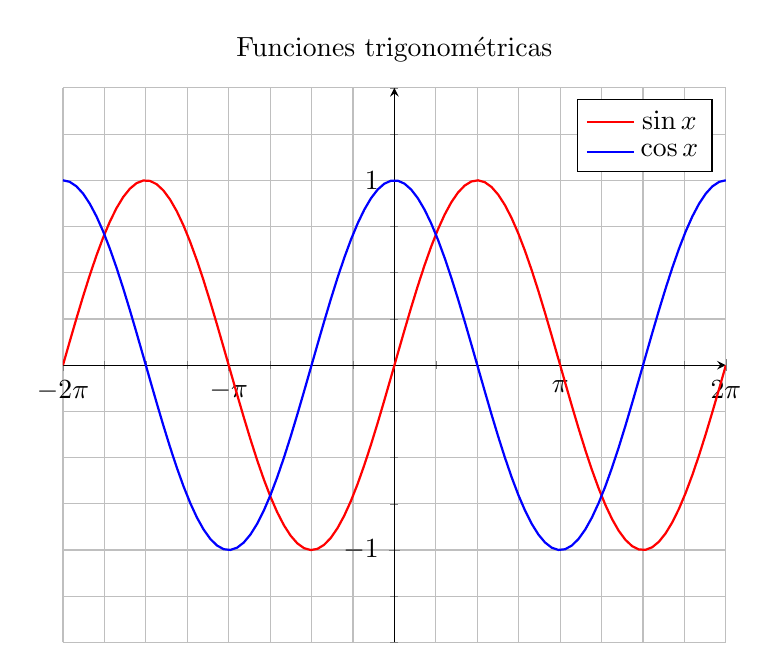
\begin{tikzpicture}
		\newcommand{\PI}{3.141592}
		\begin{axis}[
				width = 10cm,
				title = {Funciones trigonométricas},
				enlargelimits = 0,
				ymin = -1.5, ymax = 1.5,
				axis lines = middle,
				grid = both,
				ytick distance = 1,
				minor y tick num = 3,
				xtick distance = {\PI},
				minor x tick num = 3,
				xticklabels = {
					\empty,
					$-2\pi$,
					$-\pi$,
					\empty,
					$\pi$,
					$2\pi$},
				samples = 100
			]
			\addplot[red,  thick, domain=-2*\PI:2*\PI]{sin(deg(x))};
			\addlegendentry{$\sin x$}
			\addplot[blue, thick, domain=-2*\PI:2*\PI]{cos(deg(x))};
			\addlegendentry{$\cos x$}
		\end{axis}
	\end{tikzpicture}
\end{figure}

Otra razón para usar \textsc{pgfplots} es que admite gráficos en 3d y funciona de manera muy similar:
\begin{lstlisting}
\begin{axis}[
		width=8cm, samples=25,
		domain=-6:6, domain y=-6:6,
		colorbar, colormap/viridis
	]
	\addplot3[surf]{exp(-(x^2 + y^2)/25) * cos(deg(sqrt(x^2 + y^2)))};
\end{axis}
\end{lstlisting}
\begin{figure}[!h]
	\centering
	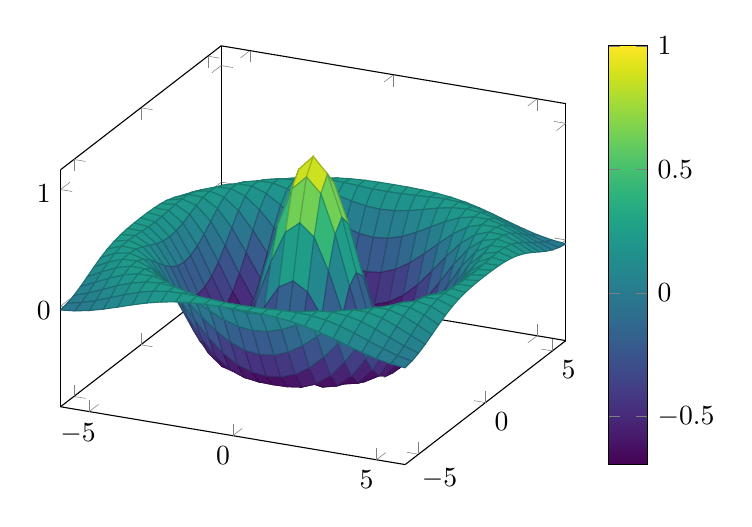
\begin{tikzpicture}
		\begin{axis}[
				width=8cm, samples=25,
				domain=-6:6, domain y=-6:6,
				colorbar, colormap/viridis
			]
			\addplot3[surf]{exp(-(x^2 + y^2)/25) * cos(deg(sqrt(x^2 + y^2)))};
		\end{axis}
	\end{tikzpicture}
\end{figure}

Aquí, \texttt{surf} es un tipo de gráfico, otro tipo es \texttt{mesh} que sólo dibuja las líneas. \texttt{colormap/viridis} determina el mapa de colores del gráfico (también hay \texttt{hot}, \texttt{cool}, \texttt{violet}, \texttt{jet} y otros). Puedes definir tu propio mapa de colores con ésta línea en la cabecera:
\begin{lstlisting}
\pgfplotsset{
	colormap={ice}{HTML(0)=(3447d4); HTML(1)=(4188ea); HTML(2)=(80dcff); HTML(3)=(a4f8ff); HTML(4)=(d2feff)}
}
--------------------------------------------------------
\begin{axis}[
		width = 6cm, hide axis, domain=-3.14:3.14,
		colormap/ice, samples = 50
	]
	\addplot[mesh, very thick]{sin(deg(x))};
\end{axis}
\end{lstlisting}
\begin{figure}[!h]
	\centering
	\begin{tikzpicture}
		\begin{axis}[
				width = 6cm, hide axis,
				colormap/ice, samples = 50
			]
			\addplot[mesh, very thick, domain=-3.14:3.14]{sin(deg(x))};
		\end{axis}
	\end{tikzpicture}
\end{figure}

Los colores del mapa anterior vienen de \url{https://www.color-hex.com/color-palette/96010}, así que corrobora que concuerdan.

En gráficos 3d también puedes usar \lstinline|view={¬theta¬}{¬phi¬}| donde \textit{theta} y \textit{phi} representan ángulos para la perspectiva del gráfico. Puede encontrar más ejemplos con más opciones aquí: \url{http://pgfplots.net/tikz/examples/all/}.

\section{Consideraciones finales}
Se recomienda chequear los manuales de \href{http://mirrors.ctan.org/graphics/pgf/base/doc/pgfmanual.pdf}{Ti$k$Z} y
\href{https://ctan.dcc.uchile.cl/graphics/pgf/contrib/pgfplots/doc/pgfplots.pdf}{\textsc{pgfplots}} para buscar más
información sobre como usarlos de manera avanzada, estoy consciente de que son manuales muy largos, pero la verdad es
que entenderás bien la dinámica básica en el primer o el segundo capítulo donde todo está bien ilustrado y documentado.
El resto de páginas es para ver cosas más avanzadas. Además existe un papel introductorio a Ti$k$Z muy completo:
\url{http://cremeronline.com/LaTeX/minimaltikz.pdf}.

Además, como puede presumir, hay un montón de paquetes y contenido que no se trató en este trabajo, y lo más probable es
que si quiere una herramienta específica para su área de investigación, entonces existe un paquete que simplifica su
implementación, por ejemplo sé que hay librerías para facilitar el diseño de circuitos eléctricos y diagramas de
Feynman.

Las partes que poseen código en el documento fueron hechas con el paquete de
\href{http://texdoc.net/texmf-dist/doc/latex/listings/listings.pdf}{\ttfamily listings}, el resto ocupa puras cosas que
este documento ya enseña, revisa
\href{https://github.com/JoseCuevasBtos/apuntes-tex/blob/master/intro-breve-latex.tex}{\textcolor{newblue}{aquí} el
código fuente} para practicar y también haz el intento de reescribir páginas de libros técnicos en \LaTeX{}, pues es sin
lugar a dudas una de las mejores herramientas para los matemáticos y físicos hoy en día.

\end{document}
